% Copyright 2007 by Till Tantau
%
% This file may be distributed and/or modified
%
% 1. under the LaTeX Project Public License and/or
% 2. under the GNU Public License.
%
% See the file doc/licenses/LICENSE for more details.

\documentclass[portuguese,10pt,xcolor=table]{bredelebeamer}
\setbeameroption{show notes}

\usepackage[brazil]{babel}
\usepackage[utf8]{inputenc}
\usepackage{times}
\usepackage{varwidth}
\usepackage{listings} % Código de programas
\usepackage{tikz}
\usepackage{pifont}
\usepackage{fourier}
\usepackage[tikz]{bclogo}
\usetikzlibrary{arrows,shapes}

\usetikzlibrary{calc,decorations.pathmorphing,patterns}
\pgfdeclaredecoration{penciline}{initial}{
	\state{initial}[width=+\pgfdecoratedinputsegmentremainingdistance,
		auto corner on length=1mm,]{
			\pgfpathcurveto%
			{% From
				\pgfqpoint{\pgfdecoratedinputsegmentremainingdistance}
				{\pgfdecorationsegmentamplitude}
			}
			{%  Control 1
				\pgfmathrand
					\pgfpointadd{\pgfqpoint{\pgfdecoratedinputsegmentremainingdistance}{0pt}}
				{\pgfqpoint{-\pgfdecorationsegmentaspect
							   \pgfdecoratedinputsegmentremainingdistance}%
							   {\pgfmathresult\pgfdecorationsegmentamplitude}
				}
			}
			{%TO 
				\pgfpointadd{\pgfpointdecoratedinputsegmentlast}{\pgfpoint{1pt}{1pt}}
			}
		}
	\state{final}{}
}



\everymath{\displaystyle}
\tikzstyle{every picture}+=[remember picture,decoration=penciline]
\DeclareTextFontCommand{\textdf}{\bfseries\color{blue!80}}
%\tikzstyle{every node}+=[decorate]
%\tikzstyle{every path}+=[decorate]
%\tikzstyle{na} = [baseline=-.5ex]

\usepackage[T1]{fontenc}

\def\lecturename{IMD0012 - Introdução às técnicas de programação}

\title{\insertlecture}

\author{Prof. Fernando Figueira\\(adaptado do material do Prof. Rafael Beserra Gomes)}

\institute{UFRN}

\subject{Arranjos Bidimensionais}

\lecture[]{Arranjos Bidimensionais}{}

\date{}

\def\exe[#1]{\color{gray}#1\color{black}}
\def\exp[#1]{\color{gray}<\textit{#1}>\color{black}}
\def\espaco{\color{gray}\hspace{0.2cm}\color{black}}
\def\espaco{\color{blue}␣\color{black}}
\def\inativo[#1]{\color{gray}#1\color{black}}

\definecolor{deepgreen}{rgb}{0,0.5,0}
\lstset{
	language=C,
	basicstyle=\footnotesize\ttfamily,
	%basicstyle=\scriptsize\ttfamily,
	keywordstyle=\footnotesize\bfseries\sffamily,
	%keywordstyle=\scriptsize\bfseries\sffamily,
	showstringspaces=false,
	numbers=left,
	numberstyle=\footnotesize,
	stepnumber=1,
	numbersep=5pt,
	tabsize=4,
	%backgroundcolor=\color{blue!05},
	backgroundcolor=\color{gray!35},
	showspaces=false,
	showtabs=false,
	stringstyle=\ttfamily\color{red!80!brown},
	commentstyle=\ttfamily\color{blue!80},
	keywordstyle=\bfseries\color{deepgreen},
	escapeinside={@}{@}
	}
	\renewcommand{\lstlistingname}{Código}
\begin{document}

\usebackgroundtemplate{%
	
\includegraphics[width=\paperwidth,height=\paperheight]{background2}
}
\begin{frame}
  \maketitle
 \begin{center}
 \tiny
Material compilado em \today.\\
  Licença desta apresentação:\\
		
\includegraphics[height=1.0cm]{by-nc-nd.png}\\
http://creativecommons.org/licenses/
	\end{center}
\end{frame}


	\def\GN[#1]{\colorbox{gray!40}{#1}}
	\def\RN[#1]{\cellcolor{red!40}#1}
	\def\BN[#1]{\colorbox{blue!40}{#1}}
	\def\ON[#1]{\colorbox{orange!40}{#1}}
	\def\WN[#1]{\colorbox{white!40}{#1}}


\section{Arranjos Bidimensionais}

	\begin{frame}[c]
		\begin{center}
			\structure{\large \insertsection}
		\end{center}
	\end{frame} 
	

	\begin{frame}{\insertsection}
		\begin{itemize}
			\item \textdf{Arranjos (array)}: conjunto de elementos identificáveis por um índice
			\item Arranjos unidimensionais: \textdf{vetores} (aula anterior)
			\item Arranjos bidimensionais: \textdf{matrizes}
		\end{itemize}
	\end{frame}	
	
	\begin{frame}{\insertsection}
		Representações de matrizes:
		\begin{itemize}
			\item Matematicamente:\\
				$$
				M = \begin{bmatrix}
					a_{11} & a_{12} & ... & a_{1m}            \\[0.3em]
					a_{21} & a_{22} & ... & a_{1m}            \\[0.3em]
					... & & \\[0.3em]
					a_{n1} & a_{n2} & ... & a_{nm}
				\end{bmatrix}
				$$
				os elementos são indexados por dois índice ($M_{ij}$) e esses começam do índice 1
		\end{itemize}
	\end{frame}	
	
	\begin{frame}{\insertsection}
		Representações de matrizes:
		\begin{itemize}
			\item Computacionalmente:
				\begin{itemize}
					\item \textbf{Em geral} há um armazenamento contíguo na memória\footnote{Se a alocação da matriz for dinâmica, há a possibilidade de alocar linhas diferentes em regiões diferentes da memória.}
					\item Os elementos são indexados por dois índices (geralmente m[i][j])
					\item O usual é primeiro índice para linha e segundo índice para coluna!
					\item Geralmente começam do índice \textbf{0}
				\end{itemize}
		\end{itemize}
	\end{frame}	
	
	\begin{frame}{Representação de matrizes na memória}
				$$
				M = \begin{bmatrix}
					1 & 2 & 3 \\[0.3em]
					4 & 5 & 6
				\end{bmatrix}
				$$

		A matriz M pode ser representada da seguinte forma na memória:
		\tiny
		 \setlength{\tabcolsep}{0pt}	
		\begin{table}
				  \begin{tabular}{|@{\hskip 0.2cm}c@{\hskip 0.2cm}|c|c|c|c|c|c|c|c|c|c|@{\hskip 0.2cm}c@{\hskip 0.2cm}|}
					\hline
					  \textbf{Endereço} & & & & & & & & & \textbf{valor} & \textbf{tipo} & \textbf{identificação}\\\hline
					  0xbffff22c & \GN[0]&\GN[0]&\GN[0]&\GN[0]&\GN[0]&\GN[1]&\GN[0]&\GN[1]& 5 & \textbf{inteiro curto} & valorIndice\\\hline
					  0xbffff22d & \BN[0]&\BN[1]&\BN[0]&\BN[0]&\BN[0]&\BN[0]&\BN[1]&\BN[0]& B & \textbf{caractere} & letra1\\\hline
					  0xbffff22e & \BN[0]&\BN[1]&\BN[0]&\BN[0]&\BN[0]&\BN[0]&\BN[1]&\BN[1]& C & \textbf{caractere} & letra2\\\hline
					  0xbffff22f & \GN[0]&\GN[0]&\GN[0]&\GN[0]&\GN[0]&\GN[0]&\GN[0]&\GN[1]& 1 & \textbf{inteiro curto} & M[0][0]\\\hline
					  0xbffff230 & \GN[0]&\GN[0]&\GN[0]&\GN[0]&\GN[0]&\GN[0]&\GN[1]&\GN[0]& 2 & \textbf{inteiro curto} & M[0][1]\\\hline
					  0xbffff231 & \GN[0]&\GN[0]&\GN[0]&\GN[0]&\GN[0]&\GN[0]&\GN[1]&\GN[1]& 3 & \textbf{inteiro curto} & M[0][2]\\\hline
					  0xbffff232 & \GN[0]&\GN[0]&\GN[0]&\GN[0]&\GN[0]&\GN[1]&\GN[0]&\GN[0]& 4 & \textbf{inteiro curto} & M[1][0]\\\hline
					  0xbffff233 & \GN[0]&\GN[0]&\GN[0]&\GN[0]&\GN[0]&\GN[1]&\GN[0]&\GN[1]& 5 & \textbf{inteiro curto} & M[1][1]\\\hline
					  0xbffff234 & \GN[0]&\GN[0]&\GN[0]&\GN[0]&\GN[0]&\GN[1]&\GN[1]&\GN[0]& 6 & \textbf{inteiro curto} & M[1][2]\\\hline
					  0xbffff235 & \BN[0]&\BN[0]&\BN[1]&\BN[1]&\BN[0]&\BN[0]&\BN[1]&\BN[0]& 2 & \textbf{caractere} & letra1\\\hline
				\end{tabular}
		\end{table}
		\normalsize
	\end{frame}

	\begin{frame}
		\begin{center}
			\structure{\large Aplicações}
		\end{center}
	\end{frame} 

	\begin{frame}{Aplicações de matrizes}
		\begin{itemize}
			\item Jogos\\
				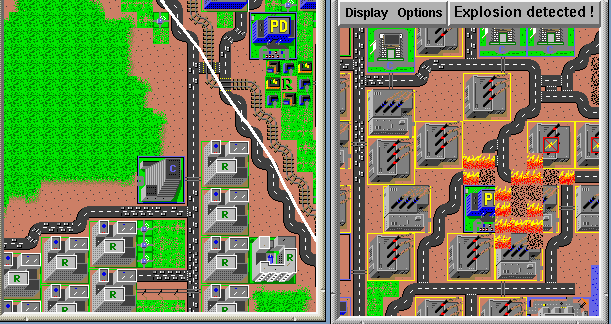
\includegraphics[height=5.2cm]{simcity.png}\\
		\end{itemize}
	\end{frame}
	\begin{frame}{Aplicações de matrizes}
		\begin{itemize}
			\item Jogos\\
				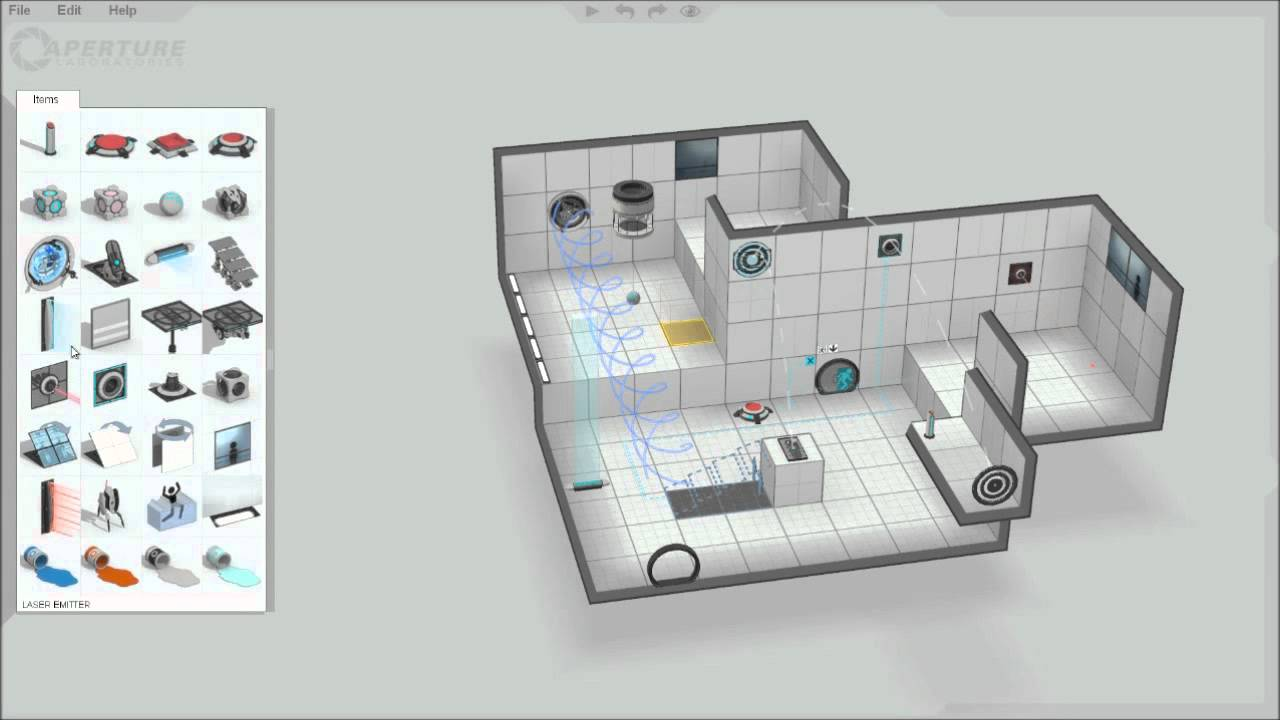
\includegraphics[height=5.2cm]{portal2.jpg}\\
		\end{itemize}
	\end{frame}

	\begin{frame}{Aplicações de matrizes}
		\begin{itemize}
			\item computação gráfica:\\
				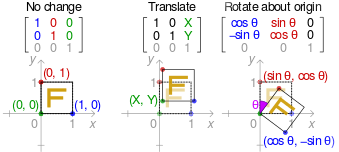
\includegraphics[height=3.0cm]{transformacao.png}
						\footnote{By Cmglee - Own work, CC BY-SA 3.0, https://commons.wikimedia.org/w/index.php?curid=35180401}
		\end{itemize}
	\end{frame}

	\begin{frame}{Aplicações de matrizes}
		\begin{itemize}
			\item resolução de outros problemas matemáticos, exemplo: regressão por mínimos quadrados\\
				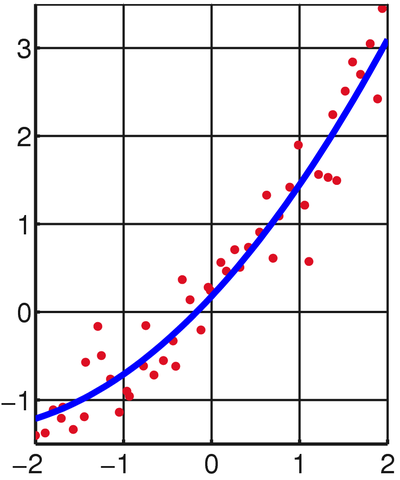
\includegraphics[height=3.2cm]{fitting.png}\\
				Regressão linear: $$
				\begin{bmatrix}
					n & \sum x_i \\
					\sum x_i & \sum x_i^2
				\end{bmatrix}
				\begin{bmatrix}
					\beta_0 \\
					\beta_1 
				\end{bmatrix}
				= 
				\begin{bmatrix}
					\sum y_i\\
					\sum x_i y_i
				\end{bmatrix}
				$$
		\end{itemize}
	\end{frame}


	\begin{frame}{Aplicações de matrizes}
		\begin{itemize}
			\item imagens digitais\\
				\tikz \node[opacity=1.0](fig1){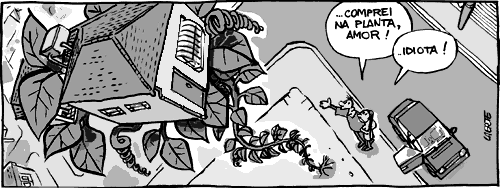
\includegraphics[width=200px]{plantaCinza.png}};
				\tikz \node[overlay,left of=fig1,draw,fill=white,opacity=0.8,right=1.04cm,above=0.4cm,minimum width=11pt, minimum height=11pt](figSelecao){ };
				\tikz \node[](fig2){
\includegraphics[width=50px]{plantaZoomEscalaCinza.png}};
				\tikz[overlay] \path[decorate,->] (figSelecao.east) edge[line width=2pt, red, bend right, dotted] (fig2.west);\\

				\tikz \node[](fig2){
\includegraphics[width=200px]{escalaCinza.png}};\\\vspace{0.5cm}
				\tikz \node[](preto){\footnotesize Preto (valor 0)};\hspace{1.1cm}
				\tikz \node[](cinza){\footnotesize Cinza (valor 127)};\hspace{0.6cm}
				\tikz \node[](branco){\footnotesize Branco (valor 255)};
				\tikz[overlay] \path[decorate,->] (preto.west) edge[line width=1pt, bend left, dotted] (fig2.west);\\
				\tikz[overlay] \path[decorate,->] (cinza.north) edge[line width=1pt, dotted] (fig2.south);\\
				\tikz[overlay] \path[decorate,->] (branco.east) edge[line width=1pt, bend right, dotted] (fig2.east);
		\end{itemize}
	\end{frame}

	\begin{frame}{Aplicações de matrizes}
		\begin{itemize}
			\item qualquer conjunto de dados n-dimensionais
				\begin{itemize}
					\item Exemplo: um conjunto de \textbf{n} coordenadas no plano cartesiano pode ser representada em uma matriz $\textbf{n} \times 2$ ou $2 \times \textbf{n}$:
						$$
						\begin{bmatrix}
							7 & 2            \\[0.3em]
							5 & 3            \\[0.3em]
							2 & 1            \\[0.3em]
							4           & 1
						\end{bmatrix}
						$$
						ou 
						$$
						\begin{bmatrix}
							7 & 5 & 2 & 4            \\[0.3em]
							2 & 3 & 1 & 1
						\end{bmatrix}
						$$
				\end{itemize}
		\end{itemize}
	\end{frame}
		
	
\section{Matrizes em C}

	\begin{frame}[c]
		\begin{center}
			\structure{\large \insertsection}
		\end{center}
	\end{frame} 

    \begin{frame}{Declarando uma matriz em C} 
		Opções:
			\lstinputlisting{declaracaoMatriz.c}
	\end{frame}

    \begin{frame}{Acesso ao elemento} 
		Basta identificar o elemento usando seus \textdf{índices} entre [] (lembre-se de que começa com 0):
			\lstinputlisting{acessoMatriz.c}
			\bcattention a maioria dos programadores usam linha como primeiro índice e coluna como segundo índice; melhor então se acostumar a pensar dessa forma
	\end{frame}

	\begin{frame}[c]
		\begin{center}
			\structure{\large Exemplo 1}
		\end{center}
	\end{frame} 
	\begin{frame}
		\begin{itemize}
			\item Escrever em uma matriz $5 \times 5$ os seguintes valores:
				\vspace{0.4cm}
				\begin{table}[]
					\centering
					\begin{tabular}{lllll}
						0 & 1 & 2 & 3 & 4 \\
						1 & 2 & 3 & 4 & 5 \\
						2 & 3 & 4 & 5 & 6 \\
						3 & 4 & 5 & 6 & 7 \\
						4 & 5 & 6 & 7 & 8
					\end{tabular}
				\end{table}
				\lstinputlisting{exemplo2.c}
		\end{itemize}
	\end{frame}	
	\begin{frame}
		\lstinputlisting{exemplo1.c}
		\only<1>{
\begin{table}
\small
\setlength{\tabcolsep}{2pt}
\begin{tabular}{|c| c| c| c| c| c| }
\hline
 \color{blue} i $\downarrow$ \color{deepgreen} $\rightarrow$ j & \color{deepgreen} 0 & \color{deepgreen} 1 & \color{deepgreen} 2 & \color{deepgreen} 3 & \color{deepgreen} 4 \\\hline 
\color{blue}\RN[ 0 ] &\RN[ 0 ] &\RN[ 1 ] &\RN[ 2 ] &\RN[ 3 ] &\RN[ 4 ] \\\hline 
\color{blue} 1 &  ? &  ? &  ? &  ? &  ? \\\hline 
\color{blue} 2 &  ? &  ? &  ? &  ? &  ? \\\hline 
\color{blue} 3 &  ? &  ? &  ? &  ? &  ? \\\hline 
\color{blue} 4 &  ? &  ? &  ? &  ? &  ? \\\hline 
\end{tabular}
\end{table}
}
\only<2>{
\begin{table}
\small
\setlength{\tabcolsep}{2pt}
\begin{tabular}{|c| c| c| c| c| c| }
\hline
 \color{blue} i $\downarrow$ \color{deepgreen} $\rightarrow$ j & \color{deepgreen} 0 & \color{deepgreen} 1 & \color{deepgreen} 2 & \color{deepgreen} 3 & \color{deepgreen} 4 \\\hline 
\color{blue}\RN[ 0 ] &\RN[ 0 ] &\RN[ 1 ] &\RN[ 2 ] &\RN[ 3 ] &\RN[ 4 ] \\\hline 
\color{blue}\RN[ 1 ] &\RN[ 1 ] &\RN[ 2 ] &\RN[ 3 ] &\RN[ 4 ] &\RN[ 5 ] \\\hline 
\color{blue} 2 &  ? &  ? &  ? &  ? &  ? \\\hline 
\color{blue} 3 &  ? &  ? &  ? &  ? &  ? \\\hline 
\color{blue} 4 &  ? &  ? &  ? &  ? &  ? \\\hline 
\end{tabular}
\end{table}
}
\only<3>{
\begin{table}
\small
\setlength{\tabcolsep}{2pt}
\begin{tabular}{|c| c| c| c| c| c| }
\hline
 \color{blue} i $\downarrow$ \color{deepgreen} $\rightarrow$ j & \color{deepgreen} 0 & \color{deepgreen} 1 & \color{deepgreen} 2 & \color{deepgreen} 3 & \color{deepgreen} 4 \\\hline 
\color{blue}\RN[ 0 ] &\RN[ 0 ] &\RN[ 1 ] &\RN[ 2 ] &\RN[ 3 ] &\RN[ 4 ] \\\hline 
\color{blue}\RN[ 1 ] &\RN[ 1 ] &\RN[ 2 ] &\RN[ 3 ] &\RN[ 4 ] &\RN[ 5 ] \\\hline 
\color{blue}\RN[ 2 ] &\RN[ 2 ] &\RN[ 3 ] &\RN[ 4 ] &\RN[ 5 ] &\RN[ 6 ] \\\hline 
\color{blue} 3 &  ? &  ? &  ? &  ? &  ? \\\hline 
\color{blue} 4 &  ? &  ? &  ? &  ? &  ? \\\hline 
\end{tabular}
\end{table}
}
\only<4>{
\begin{table}
\small
\setlength{\tabcolsep}{2pt}
\begin{tabular}{|c| c| c| c| c| c| }
\hline
 \color{blue} i $\downarrow$ \color{deepgreen} $\rightarrow$ j & \color{deepgreen} 0 & \color{deepgreen} 1 & \color{deepgreen} 2 & \color{deepgreen} 3 & \color{deepgreen} 4 \\\hline 
\color{blue}\RN[ 0 ] &\RN[ 0 ] &\RN[ 1 ] &\RN[ 2 ] &\RN[ 3 ] &\RN[ 4 ] \\\hline 
\color{blue}\RN[ 1 ] &\RN[ 1 ] &\RN[ 2 ] &\RN[ 3 ] &\RN[ 4 ] &\RN[ 5 ] \\\hline 
\color{blue}\RN[ 2 ] &\RN[ 2 ] &\RN[ 3 ] &\RN[ 4 ] &\RN[ 5 ] &\RN[ 6 ] \\\hline 
\color{blue}\RN[ 3 ] &\RN[ 3 ] &\RN[ 4 ] &\RN[ 5 ] &\RN[ 6 ] &\RN[ 7 ] \\\hline 
\color{blue} 4 &  ? &  ? &  ? &  ? &  ? \\\hline 
\end{tabular}
\end{table}
}
\only<5>{
\begin{table}
\small
\setlength{\tabcolsep}{2pt}
\begin{tabular}{|c| c| c| c| c| c| }
\hline
 \color{blue} i $\downarrow$ \color{deepgreen} $\rightarrow$ j & \color{deepgreen} 0 & \color{deepgreen} 1 & \color{deepgreen} 2 & \color{deepgreen} 3 & \color{deepgreen} 4 \\\hline 
\color{blue}\RN[ 0 ] &\RN[ 0 ] &\RN[ 1 ] &\RN[ 2 ] &\RN[ 3 ] &\RN[ 4 ] \\\hline 
\color{blue}\RN[ 1 ] &\RN[ 1 ] &\RN[ 2 ] &\RN[ 3 ] &\RN[ 4 ] &\RN[ 5 ] \\\hline 
\color{blue}\RN[ 2 ] &\RN[ 2 ] &\RN[ 3 ] &\RN[ 4 ] &\RN[ 5 ] &\RN[ 6 ] \\\hline 
\color{blue}\RN[ 3 ] &\RN[ 3 ] &\RN[ 4 ] &\RN[ 5 ] &\RN[ 6 ] &\RN[ 7 ] \\\hline 
\color{blue}\RN[ 4 ] &\RN[ 4 ] &\RN[ 5 ] &\RN[ 6 ] &\RN[ 7 ] &\RN[ 8 ] \\\hline 
\end{tabular}
\end{table}
}

	\end{frame}
	
	\begin{frame}[c]
		\begin{center}
			\structure{\large Exemplo 2}
		\end{center}
	\end{frame} 
	\begin{frame}
		\begin{itemize}
			\item Ler do usuário uma matriz $5 \times 5$:
				\lstinputlisting{exemplo3.c}
		\end{itemize}
	\end{frame}	
		
	\begin{frame}
		\begin{alertblock}{\ding{46} Exercício em sala}
			Declare uma matriz $5 \times 5$ e preencha com uma matriz triangular superior. Depois escreva os valores da matriz na tela.
			\begin{table}[]
				\centering
				\begin{tabular}{lllll}
					1 & 1 & 1 & 1 & 1 \\
					0 & 1 & 1 & 1 & 1 \\
					0 & 0 & 1 & 1 & 1 \\
					0 & 0 & 0 & 1 & 1 \\
					0 & 0 & 0 & 0 & 1
				\end{tabular}
			\end{table}
		\end{alertblock}
	\end{frame}
	
	\begin{frame}
		\begin{alertblock}{\ding{46} Exercício em sala}
			Declare uma matriz $5 \times 5$ e preencha com a seguinte matriz de tal forma que:
			\begin{itemize}
				\item A primeira linha é 1, 2, 3, 4, 5
				\item Qualquer outro número da matriz, exceto da última coluna, é igual à soma do número acima com o número à nordeste
				\item O número da última coluna (exceto o da primeira linha) é igual ao da penúltima coluna
			\end{itemize}
			Depois escreva os valores da matriz na tela.
			\begin{table}[]
				\centering
				\begin{tabular}{lllll}
					1 & 2 & 3 & 4 & 5 \\
					3 & 5 & 7 & 9 & 9 \\
					8 & 12 & 16 & 18 & 18 \\
					20 & 30 & 34 & 36 & 36 \\
					50 & 64 & 70 & 72 & 72
				\end{tabular}
			\end{table}
		\end{alertblock}
	\end{frame}

	\iffalse
	\begin{frame}
		\begin{alertblock}{\ding{46} Exercício em sala}
			\footnotesize	Declare uma matriz $30 \times 31$ de \textbf{char} e preencha com valores digitados pelo usuário (30 linhas). Esses valores representam um mapa da cidade do jogo simulador de cidades: '\#' significa um prédio, ' ' um espaço vazio e '-' uma rua. Depois de um desastre \bomb algumas ruas foram destruidas. Conecte duas ruas que estiverem separadas por um único espaço na horizontal ou vertical.
			Exemplo reduzido abaixo:
			\begin{table}[]
				\centering
				\begin{tabular}{lllll}
					-  &\#  &\#  &  &  \\
					 & \# & \# & \# &  \\
					- & - &   & - &  \\
					 & \# & \# & \# & - \\
					 \# & \# & \# & \# & \#
				\end{tabular}
			\end{table}
			O resultado será:
			\begin{table}[]
				\centering
				\begin{tabular}{lllll}
					-  &\#  &\#  &  &  \\
					- & \# & \# & \# &  \\
					- & - & - & - &  \\
					 & \# & \# & \# & - \\
					 \# & \# & \# & \# & \#
				\end{tabular}
			\end{table}
		\end{alertblock}
	\end{frame}
	\fi



\end{document}

